\subsection{The Z algorithm}
The Z algorithm is a simple yet important algorithm in string matching and is sometimes referred to as a fundamental preprocessing step.\cite{Gusfield1997AlgorithmsOS} The Z algorithm is used to preprocess a string $S$ and results in an array of $Z_i(S)$ values that alone can be used to do string matching in linear time but is also used in the preprocessing step of other algorithms like the Knuth-Morris-Pratt and Boyer-Moore algorithms. Sometimes it is the entire basic string matching algorithm that the array of $Z_i(S)$-values results in that is called the Z algorithm, but here Z algorithm refers only to finding the $Z_i(S)$ values. 

In the following, the Z algorithm and the definitions required to understand it are introduced. The Z algorithm is explained in detail, before explaining how it can be used for the (KMP???) and Boyer-Moore algorithms. 

First off, consider the definition of $Z_i(S)$ for a given string $S$. When the string is clear by context, $Z_i$ can be used instead of $Z_i(S)$. 

\begin{itemize}
    \item[] \textbf{Definition} Given a string $S$ and a position $i>1$ let $Z_i(S)$ denote the length of the longest substring of $S$ that starts at $i$ and matches a prefix of $S$. 
\end{itemize}

This means that $Z_i$ is how far a substring starting in position $i$ can be read while matching the beginning of $S$. There is a nice way of visualising the $Z_i$ values for a given string, namely $Z$-boxes. Consider figure \ref{fig:z_boxes}, where the string $S$ is represented by a long horizontal line and for each position $x$ up to $i$ where $Z_x>0$, the substring starting at $x$ of length $Z_x$ is shown as a box. In this manner, each box represents a substring that matches a prefix of $S$. 

For a given position $i$, there may be many $Z$-boxes starting at a position less than $i$, so it is useful to have the following two definitions:

\begin{itemize}
    \item[] \textbf{Definition} For any position $i>1$ where $Z_i>0$ the $Z$-box at $i$ is defined as the substring starting at $i$ of length $Z_i$, ending in position $i+Z_i-1$. 
    \item[] \textbf{Definition} For every $i>1$, $r_i$ is the right-most endpoint of the \textit{$Z$-boxes} that begin at or before position $i$ and $l_i$ is the left end of one such $Z$-box. If there are more than one option, $l_i$ can refer to any one of them. 
\end{itemize}

\begin{figure}[t]
    \centering
    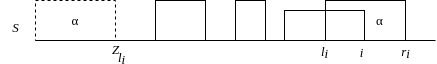
\includegraphics[width=.9\textwidth]{LaTeX/Figures/Zalg/zboxes.png}
    %\includesvg{LaTeX/Figures/Zalg/Zalg.drawio(1)}
    \caption{The solid boxes represent a substring of $S$ that matches a prefix of $S$, called $Z$-boxes. For a given position $i$, the right-most end of any $Z$-box beginning at or before $i$ is defined as $r_i$, the substring in that $Z$-box is $\alpha$, and the left end is $l_i$. }
    \label{fig:z_boxes}
\end{figure}

These definitions are enough to define and understand the Z algorithm. The Z algorithm works inductively by assuming for a position $i$ that the algorithm has correctly computed the $Z_x$ values for $x$ from 2 up to $i-1$ as well as the $r_{i-1}$ and $l_{i-1}$ values. It uses these to compute the next $Z_i$, $r_i$ and $l_i$ values. The idea is to use the concept of Z-boxes to infer information about the next $Z_i$ value and thus compute every $Z_i$ value in linear time. 

The Z algorithm divides into four different cases, which are most easily understood by following figure \ref{fig:Zalg}. 

Even though $r_i$ and $l_i$ are defined for each position $i$, the algorithm requires only the right-most $r$ value and its corresponding $l$ value and updates them when finding a $Z$-box that ends at a later position. This is why the algorithm uses a single variable to denote $r$ and $l$. 

\begin{algorithm}
\caption{Z algorithm}\label{alg:z_alg}
\begin{algorithmic}
\State Initialise $r=l=0$ and $Z_i=0$ for all $i$. 
\State For each position $k$, compute $Z_k$ and update $r$ and $l$ as follows
\For{$k=2..|S|$}
\If{$k>r$} \Comment{Case 1}
    \State Compute $Z_k$ explicitly by comparing characters from position $k$ to the \State beginning of $S$ until a mismatch is found. 
    \State $Z_k:=length\_of\_match$
    \State $l:=k$
    \State $r:=k+Z_k-1$
\ElsIf{$k\leq r$}
    \State Let $k':=l-k+1$ and $\beta:=S[k..r]$
    \If{$Z_{k'}<|\beta|$} \Comment{Case 2a}
        \State $Z_k:=Z_{k'}$
        \State $r$ and $l$ unchanged. 
    \ElsIf{$Z_{k'}>|\beta|$} \Comment{Case 2b}
        \State $Z_k:=|\beta|$
        \State $r$ and $l$ unchanged. 
    \ElsIf{$Z_{k'}=|\beta|$} \Comment{Case 2c}
        \State The substring $\beta$ matches a prefix of $S$ but might match longer than $Z_{k'}$. \State Match characters of $S$ from position $|\beta|+1$ with position $r+1$ until a \State mismatch occurs, say at position $q\geq r+1$. Then update
        \State $Z_k:=q-k$
        \State $r:=q-1$
        \State $l:=k$
    \EndIf
\EndIf
\EndFor
\end{algorithmic}
\end{algorithm}


\begin{figure}[t]
\centering
\begin{subfigure}{0.9\textwidth}
    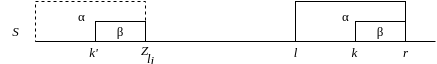
\includegraphics[width=\textwidth]{LaTeX/Figures/Zalg/Zalg1.png}
    \caption{The substring $S[k..r]$, labelled $\beta$, also occurs at position $k'$ of $S$}
    \label{fig:Zalg1}
\end{subfigure}
\hfill
\begin{subfigure}{0.9\textwidth}
    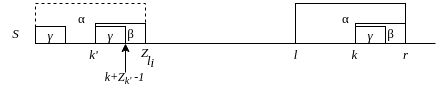
\includegraphics[width=\textwidth]{LaTeX/Figures/Zalg/Zalg2a.png}
    \caption{Case 2a. The longest substring, $\gamma$, starting at $k'$ matching a prefix of $S$ is shorter than $\beta$. }
    \label{fig:Zalg2a}
\end{subfigure}
\hfill
\begin{subfigure}{0.9\textwidth}
    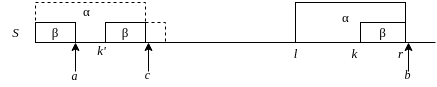
\includegraphics[width=\textwidth]{LaTeX/Figures/Zalg/Zalg2b.png}
    \caption{Case 2b. The longest substring starting at $k'$ matching a prefix of $S$ extends beyond the $Z$-box, meaning character $b$ and $c$ and thus $a$ and $b$ are a mismatch. }
    \label{fig:Zalg2b}
\end{subfigure}
\hfill
\begin{subfigure}{0.9\textwidth}
    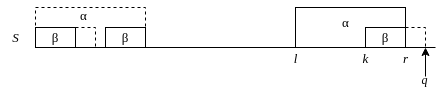
\includegraphics[width=\textwidth]{LaTeX/Figures/Zalg/Zalg2c.png}
    \caption{Case 2c. The length of longest substring starting at $k'$ matching a prefix of $S$ is exactly the length of $\beta$, meaning the match could extend further than $r$. }
    \label{fig:Zalg2c}
\end{subfigure}
\caption{The various cases of the Z algorithm. }
\label{fig:Zalg}
\end{figure}

\subsubsection{Explanation of the Z algorithm}
In order to work inductively, the algorithm must start by computing the first values for $Z_k$, $r$ and $l$. This is covered in case 1, where it explicitly compares $S[2..|S|]$ with $S[1..|S|]$ until a mismatch is found. In general, case 1 ensures that when position $k$ is not inside an already found $Z$-box, the algorithm will look for new boxes, not missing any. 

There are several cases when position $k$ is inside a $Z$-box. Denote the substring in the $Z$-box by $\alpha=S[l..r]$, which matches a prefix of $S$. This means character $S(k)$ matches position $k'=k-l+1$ of $S$. Similarly, the substring $\beta=S[k..r]$ matches the substring $S[k'..Z_l]$, see figure \ref{fig:Zalg1}. Logically, the substring beginning at position $k$ must then match a prefix of $S$ at least the minimum of $|\beta|$ and $Z_{k'}$. 

When $Z_{k'}<|\beta|$, called case 2a in the algorithm, the smaller substring $\gamma=S[k'..k'+Z_{k'}-1]$ is a maximal length substring that matches a prefix of $S$ and therefore the substring starting at position $k$ can match exactly $Z_{k'}$ characters at the beginning of $S$. 

When $Z_{k'}>|\beta|$, called case 2b in the algorithm, $\beta$ matches all characters in $S[k'..Z_l]$, but $S(|\beta|+1)=:a$ cannot match $S(k+|\beta|+1)=:b$. Why? Because by definition, $\alpha$ is a maximal length substring that matches a prefix of $S$, which means that there must be a mismatch at the end of the $Z$-box starting at position $l$ with the character at position $Z_l+1$, $c:=S(Z_l+1)$. And since $Z_{k'}>|\beta|$, the character $c$ matches the character $a$. Altogether this means that $a=c$ and $c\neq b$ implies $a\neq b$, i.e. that $S(|\beta|+1)$ mismatches $S(k+|\beta|+1)$. In this case, $Z_k=Z_{k'}$ and no more. 

Following the logic above, when $Z_{k'}=|\beta|$, the substring $\beta$ matches $S[k'..Z_l]$. But now $Z_{k'}=|\beta|$ only implies that $S(Z_{k'}+1)$ mismatches $S(k'+Z_{k'}+1$, i.e. $a\neq c$. From above, $c\neq b$ still holds, but now $a=b$ is a possibility, so start matching from those two characters beyond the current $Z$-box $\alpha$. When the next mismatch is found at position $q\geq r+1$, update $Z_k$, $r$ and $l$ as described in the algorithm, since a new right-most $Z$-box has been found. 

\subsection{More advanced string matching algorithms}

Using the Z algorithm, a basic algorithm that runs in linear time is apparent: given a pattern $P$ and text $T$, find all $Z_i$ values in $P\$T$ where $\$$ is a character not in the alphabet. All values are at most $n=|P|$ and when a position $i$ has $Z_i=n$, then the substring starting at $i$ in $P\$T$ matches $P$. This basic algorithm runs in linear time, since the Z algorithm runs in linear time. A proof for the linear time complexity of the Z algorithm is given in \cite{Gusfield1997AlgorithmsOS}. 

There exist many more advanced string matching algorithms than this basic one and these will be explored in the following. 
